\documentclass{article}
\usepackage[utf8]{inputenc}
\usepackage{float}
\usepackage{listings}
\lstset{language=Python}
\lstset{frame=lines}
\lstset{label={lst:code_direct}}
\lstset{basicstyle=\footnotesize}
\title{Machine Learning 1: Foundations - Exercise Sheet 1}
\author{Gur Amrit Pal Singh }
\date{\today}
\usepackage{natbib}
\usepackage{graphicx}
\begin{document}
\maketitle

\noindent\textbf{Question 3}\newline
\textbf{a):} A scatter plot where the x-axis is the height of the citizens and the y-axis is the weight of the citizens.
\begin{figure}[H]
\centering
    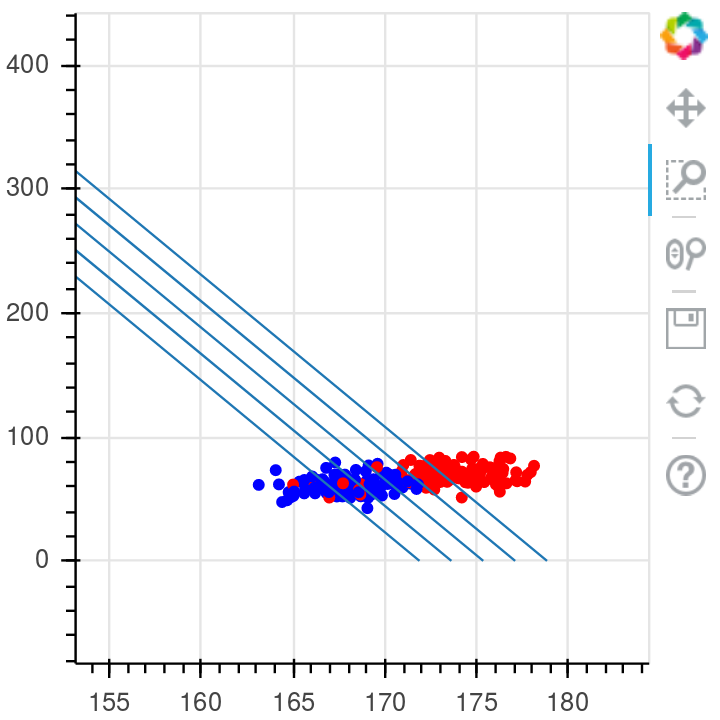
\includegraphics[scale=0.6]{Question3.png}
\caption{Scatter Plot}
\label{fig:scatter_plot1}
\end{figure}
\begin{lstlisting}[language=Python]
import matplotlib.pyplot as plt
import pandas as pd

data = pd.read_csv("DWH_Training.csv",names = ["Height", "Weight", "Gender"])
groups = data.groupby('Gender')
fig, ax = plt.subplots()
for name, group in groups:
    if(name==-1):
        ax.plot(group.Height, group.Weight, marker='*',linestyle='', ms=12, label='Female')
    else:
        ax.plot(group.Height, group.Weight, marker='*', linestyle='', ms=12, label='Male')
ax.legend()
plt.show()
\end{lstlisting}\\
\\~\\
\\~\\
\textbf{b):} A horizontal line which best separates male and female citizens.
\begin{figure}[H]
\centering
    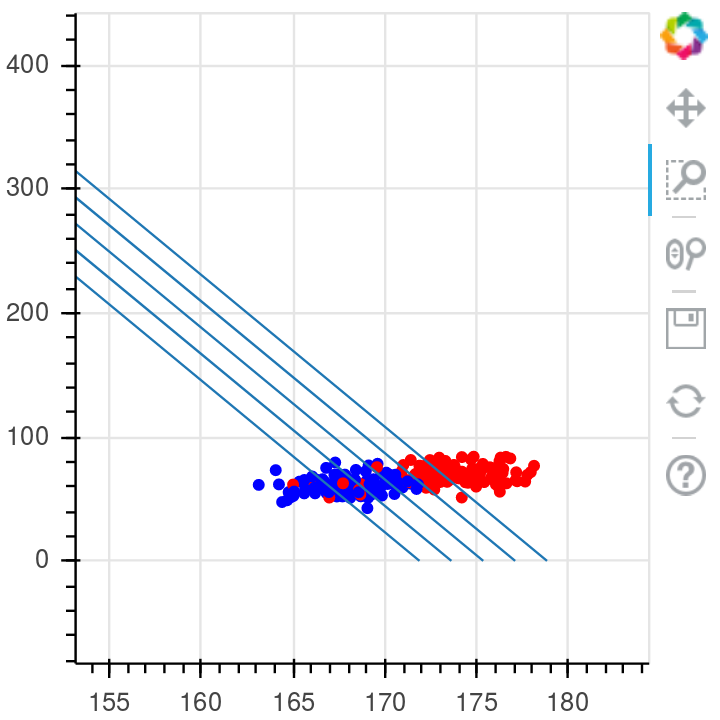
\includegraphics[scale=0.6]{Question4.png.png}
\caption{Scatter Plot with Horizontal Line}
\label{fig:scatter_plot2}
\end{figure}
\begin{lstlisting}[language=Python]
import matplotlib.pyplot as plt
import pandas as pd
import matplotlib.lines as mlines

data = pd.read_csv("DWH_Training.csv",names = ["Height", "Weight", "Gender"])

groups = data.groupby('Gender')
fig, ax = plt.subplots()
for name, group in groups:
    if(name==-1):
        ax.plot(group.Height, group.Weight, marker='*', linestyle='', ms=12, label='Female')
    else:
        ax.plot(group.Height, group.Weight, marker='*', linestyle='', ms=12, label='Male')
ax.legend()
line_hor = mlines.Line2D([0, 178], [66,66], color='r',linestyle='dashed')
ax.add_line(line_hor)

plt.show()
\end{lstlisting}
\\~\\
\\
\textbf{c):} One of the parents of Mr Duck Tales weighs 62 kg we can not say whether the parent is Mr Duck Tales father or mother without knowing the height of the person. This can be justified with the graph showing below. The black line passes through both the males and females that weigh 62 kg, so without the input of the height we can't make any comment.
\begin{figure}[H]
\centering
    \includegraphics[scale=0.6]{simple_scatter_plot_c.png}
\caption{Scatter Plot with Horizontal Line showing people who weigh 62 kg}
\label{fig:scatter_plot3}
\end{figure}
\\~\\
\\
\textbf{d):} A vertical line which best separates male and female citizens.
\begin{figure}[H]
\centering
    \includegraphics[scale=0.6]{simple_scatter_plot_ver.png}
\caption{Scatter Plot with Horizontal Line}
\label{fig:scatter_plot4}
\end{figure}
\begin{lstlisting}[language=Python]
import matplotlib.pyplot as plt
import pandas as pd
import matplotlib.lines as mlines

data = pd.read_csv("DWH_Training.csv",names = ["Height", "Weight", "Gender"])

groups = data.groupby('Gender')
fig, ax = plt.subplots()
for name, group in groups:
    if(name==-1):
        ax.plot(group.Height, group.Weight, marker='*', linestyle='', ms=12, label='Female')
    else:
        ax.plot(group.Height, group.Weight, marker='*', linestyle='', ms=12, label='Male')
ax.legend()
line_ver = mlines.Line2D([171, 171], [0, 90], color='g',linestyle='dashed')
ax.add_line(line_ver)

plt.show()
\end{lstlisting}
\\~\\
\\
\textbf{e):} One of the siblings of Mrs Minnie Mouse is 181cm tall. The sibling must be female as show in the graph below, every person taller than 174cm is a female (shown by green dashed line) . So we can pretty much guarantee that the sibling is a female.
\begin{figure}[H]
\centering
    \includegraphics[scale=0.6]{simple_scatter_plot_e.png}
\caption{Scatter Plot with Horizontal Line showing people taller than 174 cm}
\label{fig:scatter_plot5}
\end{figure}
\\~\\
\\
\textbf{f):} The line which best separates male and female citizens.
\begin{figure}[H]
\centering
    \includegraphics[scale=0.6]{simple_scatter_plot_best.png}
\caption{Scatter Plot with Line which best separates the citizens}
\label{fig:scatter_plot6}
\end{figure}
\begin{lstlisting}[language=Python]
import matplotlib.pyplot as plt
import pandas as pd
import matplotlib.lines as mlines

data = pd.read_csv("DWH_Training.csv",names = ["Height", "Weight", "Gender"])
print(data)

groups = data.groupby('Gender')
fig, ax = plt.subplots()
for name, group in groups:
    if(name==-1):
        ax.plot(group.Height, group.Weight, marker='*', linestyle='', ms=12, label='Female')
    else:
        ax.plot(group.Height, group.Weight, marker='*', linestyle='', ms=12, label='Male')
ax.legend()
line_ver = mlines.Line2D([170, 180], [95, -200], color='g',linestyle='dashed')
ax.add_line(line_ver)

plt.show()

\end{lstlisting}
\\~\\
\\
\textbf{f):} Using the best fit line we would classify the Donald Duck's cousin who weighs 52kg and is 179 cm tall to be a female. But if we use b) graph to classify him/her, we would classify him/her as a male, and using the d graph we would classify him/her as female.
\\~\\
\\
\noindent\textbf{Question 4}\newline
\textbf{a):} 
\end{document}